%
% qam.tex -- Quadratur-Amplituden-Modulation mit Matrizen und Vektorgeometrie
%
% (c) 2020 Prof Dr Andreas Müller, Hochschule Rapperswil
%
\section{Quadratur-Amplituden-Modulation
\label{section:quadratur-amplituden-modulation}}
\rhead{Quadratur-Amplituden-Modulation}
Um ein zeitabhängiges Signal drahtlos zu übertragen, muss es auf
ein hochfrequentes Trägersignal aufmoduliert werden.
Wie macht man das und wie kann man das ursprüngliche Signal
wiedergewinnen?
Eine besonders flexible Methode, die sogenannte
Quadratur-Amplituden-Modu\-lation, lässt sich mit Hilfe von Vektorgeometrie
und Drehmatrizen besonders leicht verstehen.


%
% amplitudenmodulation.tex
%
% (c) 2020 Prof Dr Andreas Müller, Hochschule Rapperswil
%
\subsection{Amplitudenmodulation
\label{subsection:amplitudenmodulation}}
Die Technik der Amplitudenmodulation geht auf die Anfangszeit des
Radios zurück.
Um ein zeitabhängiges Audio-Signal $I(t)$ mit Frequenzen von typischwerweise
wenigen hundert Herz oder wenigen Kilohertz drahtlos zu übertragen,
verändert man die Amplitude eines Trägersignals von mehreren hundert
Kilohertz oder mehr und leitet es zu einer Antenne.
Diese strahlt dann eine entsprechend oszillierendes elektromagnetisches
Feld ab, welches von einem Empfänger aufgefangen und wieder hörbar gemacht
werden kann.

\begin{figure}
\centering
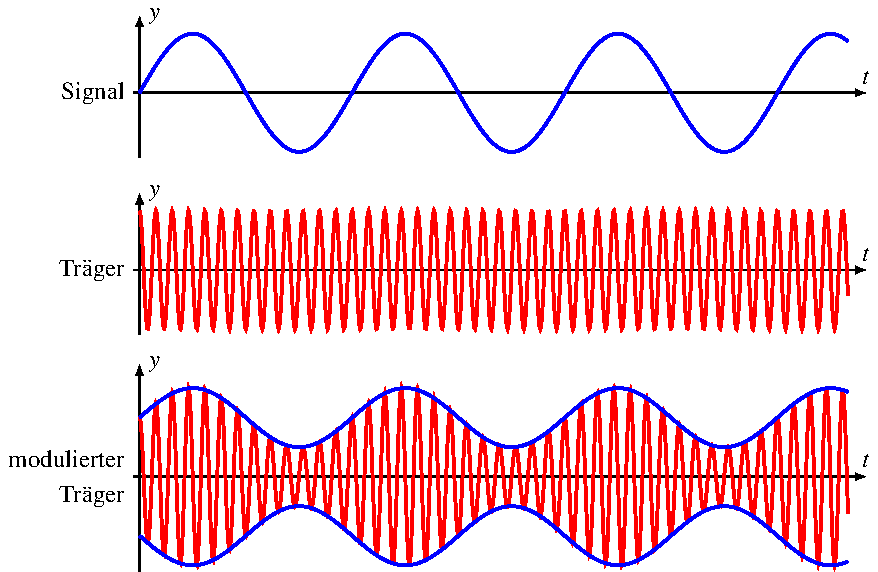
\includegraphics{applications/qam/am.pdf}
\caption{Amplitudenmodulation eines Signals $I(t)$ auf eine
Trägerfrequenz $\cos\omega t$.
Die Amplitude des Trägers wird im Takt des Signals verändert.
\label{figure:qam:am}}
\end{figure}

In Abbildung~\ref{figure:qam:am} wird die Amplitude des Träger
$\cos\omega t$ mit der Kreisfrequenz $\omega$ wird im Takt des
Signals verändert,
konkret wird der Träger mit $1+I(t)$ multipliziert,
das übermittelte Signal ist also
\begin{equation}
(1+I(t)) \cos\omega t.
\end{equation}
Ein so moduliertes Signal ist besonders leicht zu demodulieren.
Es reicht, das Signal gleichzurichten und verbleibenden Reste
der Trägerfrequenz sowie die konstente Komponten auszufiltern.
Ein
\begin{figure}
\centering
\begin{tikzpicture}
\node at (0,0) {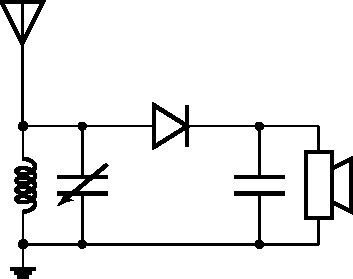
\includegraphics{applications/qam/detektor.pdf}};
\node at (8,0) {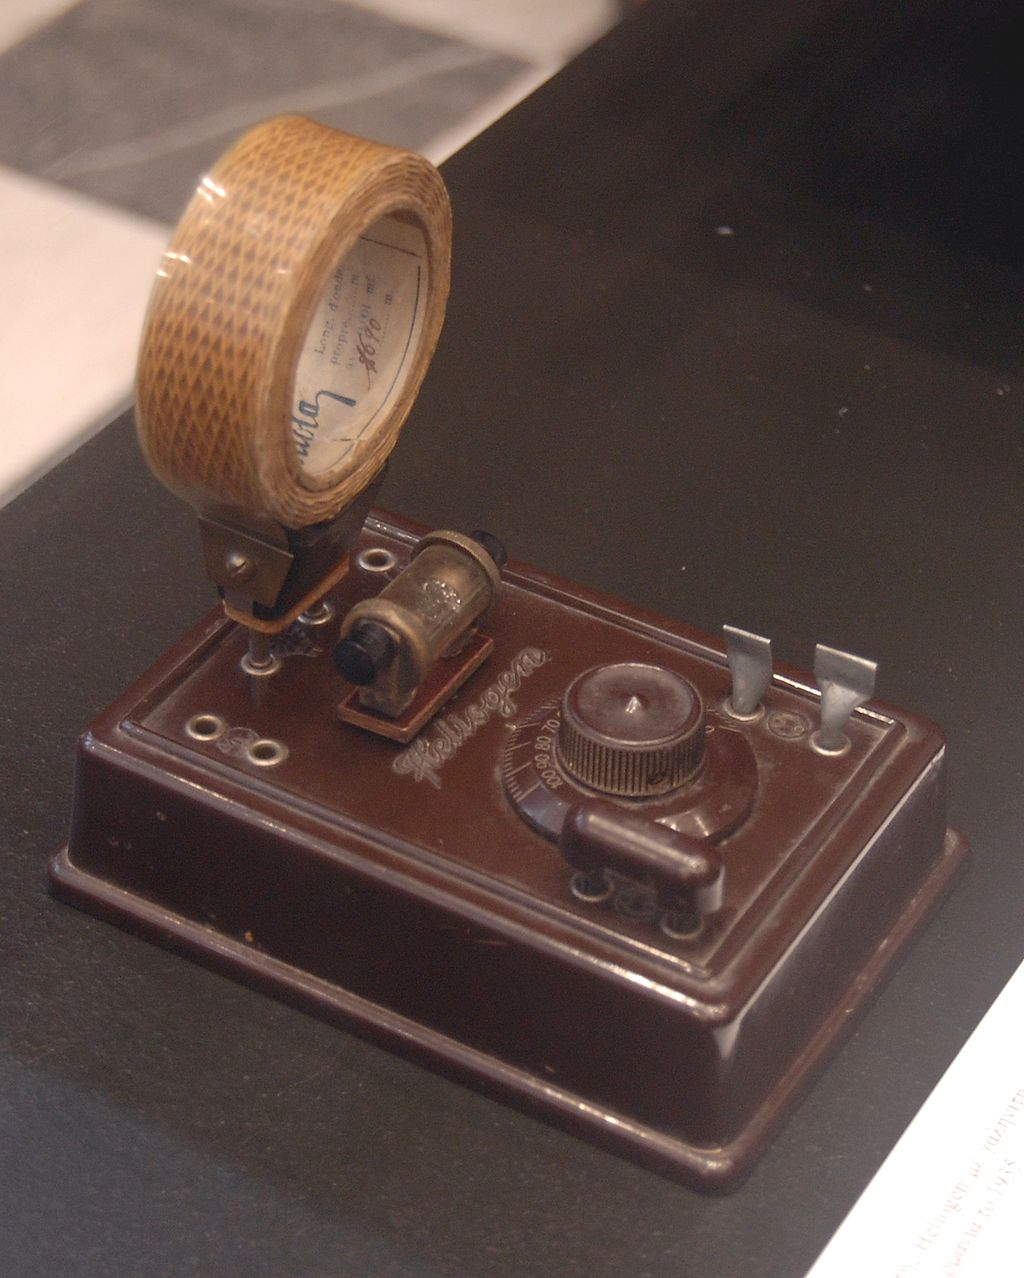
\includegraphics[width=6cm]{applications/qam/detektor.jpg}};
\end{tikzpicture}
\caption{Ein Detektorradio besteht aus einem einstellbaren
Schwingkreis zur Auswahl der Trägerfrequenz, einer Diode zur
Gleichrichtung und einem Kondensator zur Filterung der Überreste
des Trägers.
Bei starken Sendern kann das niederfrequente Tonsignal ohne
Verstärkung mit einem Kopfhörer abgehört werden.
\label{figure:qam:detektor}}
\end{figure}
Die konstante Komponente (der Summand $1$) ist nicht wirklich
interessant und dient nur einer leichter verständlichen Darstellung
in Abbildung~\ref{figure:qam:am}, wir werden sie in Zukunft 
ignorieren und nur noch das modulierte Signal $I(t)\cos\omega t$
betrachten.

Mit dieser Methode kann man zu jeder Zeit $t$ einen einzelnen
Wert $I(t)$ übermitteln.
Für die Praxis ist das schon bei Audiosignalen oft ungenügend, man
möchte doch mindestens die beiden Stereokanäle eines qualitativ
hochwertigen Signals übertragen können.

Die zweite Schwierigkeit ist die Frage, warum wir $\cos\omega t$
dem ebenfalls möglichen Träger $\sin\omega t$ vorziehen sollen.
Die beiden unterscheiden sich nur um eine Phasenverschiebung
von $90^\circ$, die für die oben beschriebene Modulation und
Demodulation bedeutungslos ist.







%
% zweidimensionale.tex
%
% (c) 2020 Prof Dr Andreas Müller, Hochschule Rapperswil
%
\subsection{Zweidimensionale Signale
\label{subsection:qam:zweidimensional}}
Wir suchen also nach einem Verfahren, mit welchem wir nicht nur
ein einzelnes zeitabhängiges Signal $I(t)$ übertragen können, sondern
auch noch ein zweites Signal, welches wir mehr oder weniger aus
historischen Gründen $Q(t)$ nennen wollen\footnote{Das Signal $I(t)$
heisst auch die In-phase-Komponente und $Q(t)$ Quadratur-Komponente}.
Man kann sich die beiden Signale zum Beispiel also die beiden
Stereokanäle eines Audiosignals vorstellen.
Wir stellen uns die beiden Komponenten als untrennbar zusammengehörig
vor, es ist daher sinnvoll, sie als zweidimensionalen Vektor
\[
\vec{v}(t)
=
\begin{pmatrix}I(t)\\Q(t)\end{pmatrix}
\]
zu schreiben.
Dieser Vektor beschreibt zu jeder Zeit $t$ einen Punkt in der
$I$-$Q$-Ebene.
Zu verschiedenen Zeiten beschreibt $\vec{v}(t)$ eine Kurve
in der Ebene.
Mit einem Oszilloskop im X-Y-Modus kann man den Vektor
sichtbar machen.
Zum Beispiel führt das Signal
\begin{equation}
I(t) = \cos t,\quad
Q(t) = \sin 3t
\qquad
\Rightarrow
\qquad
\vec{v}(t)
=
\begin{pmatrix}
\cos t\\
\sin 3t
\end{pmatrix}
\label{eqn:qam:liss1}
\end{equation}
auf die in Abbildung~\ref{figure:qam:lissajous} dargestellte Kurve.
\begin{figure}
\centering
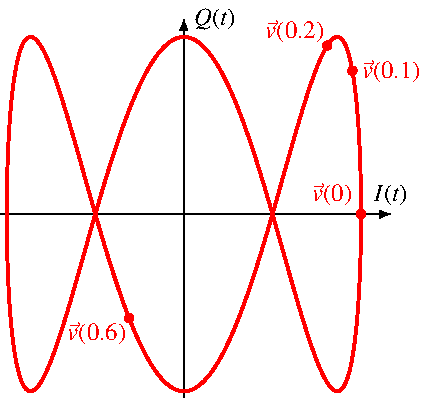
\includegraphics[width=0.48\hsize]{applications/qam/images/lissajous.pdf}
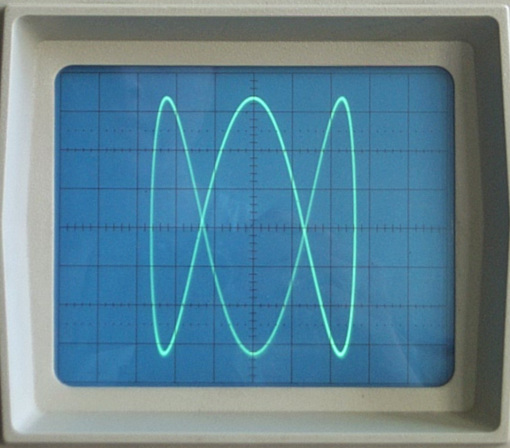
\includegraphics[width=0.48\hsize]{applications/qam/images/lissajous.jpg}
\caption{Lissajous-Figur des zweidimensionalen Signals
\eqref{eqn:qam:liss1} kann auf einem Oszilloskop im X-Y-Modus
sichtbar gemacht werden.
\label{figure:qam:lissajous}}
\end{figure}
Solche Kurven sind bekannt als Lissajous-Figuren.
Mit komplizierteren Funktion $I(t)$ und $Q(t)$ kann fast jede
Linienzeichnung auf den Schirm des Oszilloskops gezaubert werden,
wie zum Beispiel auch die Internet ``Kunstform'' der Oscilloscope
Music (\url{https://www.youtube.com/watch?v=qnL40CbuodU}) zeigt.
In Abbildung~\ref{figure:qam:pilze} werden zum Beispiel Pilze und
ein Schmetterling mit zwei geeigneten Funktionen $I(t)$ und $Q(t)$
gezeichnet.

\begin{figure}
\centering
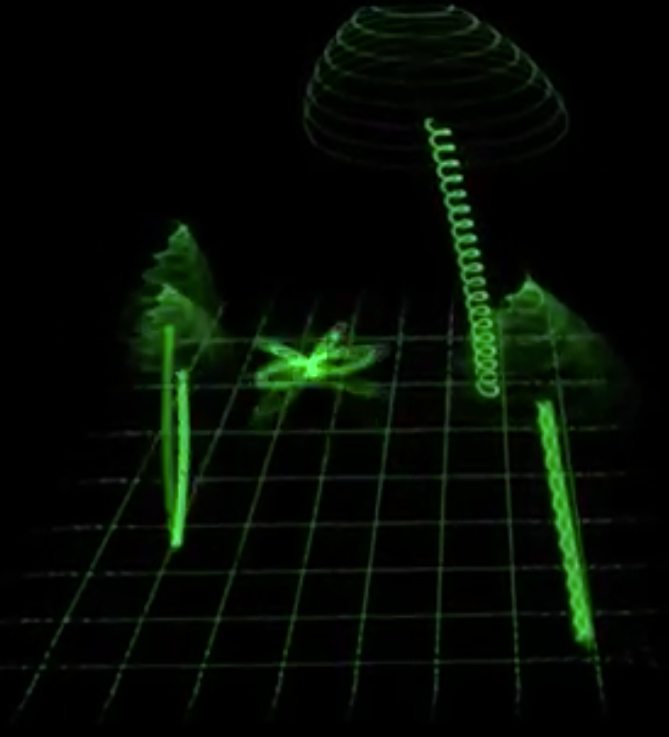
\includegraphics[width=0.5\hsize]{applications/qam/images/pilze.png}
\caption{Pilze und ein Schmetterling gezeichnet von zwei Signalen
$I(t)$ und $Q(t)$ aus dem Video \url{https://youtu.be/rtR63-ecUNo}
\label{figure:qam:pilze}}
\end{figure}




%
% modulation.tex
%
% (c) 2020 Prof Dr Andreas Müller, Hochschule Rapperswil
%
\subsection{Modulation zweidimensionaler Signale
\label{subsection:modulation}}
Wir streben jetzt an, ein zweidimensionales Signal
\[
\vec{v}(t)
=
\begin{pmatrix}I(t)\\Q(t)\end{pmatrix}
\]
drahtlos zu übertragen und müssen zu diesem Zweck ein geeignetes
Modulationsverfahren finden.

\begin{figure}
\centering
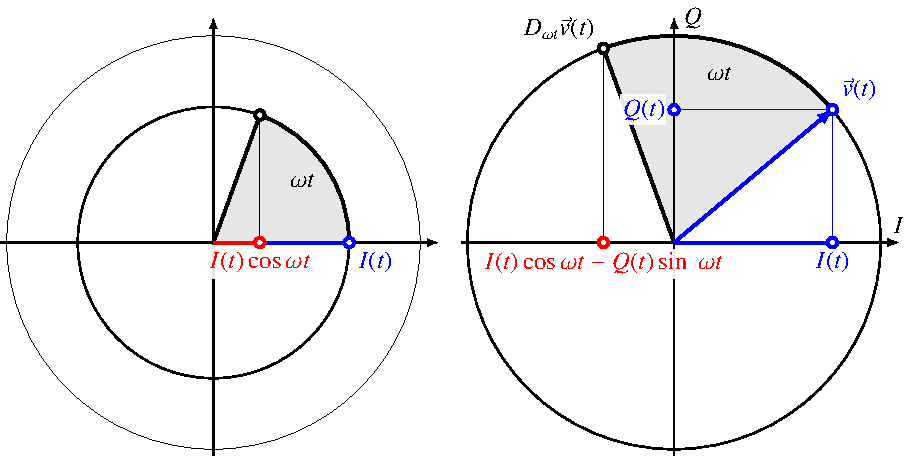
\includegraphics{applications/qam/images/icos.pdf}
\caption{Modulation des Signals $I(t)$ als Drehung um den Winkel $\omega t$
auf einem Kreis mit Radius $I(t)$.
\label{qam:figure:icos}}
\end{figure}
Mit nur dem einen Signal $I(t)$ haben wir $I(t)\cos\omega t$ als moduliertes
Signal gewählt.
Geometrisch können wir das auf einem Kreis mit Radius $I(t)$ als Drehung
um den Winkel $\omega t$ mit anschliessender Projektion auf die horizontale
Achse verstehen (Abbildung~\ref{qam:figure:icos} links).

Es ist daher naheliegend, für die Modulation des zweidimensionalen Signals
ebenfalls eine Drehung um den Winkel $\omega t$ zu verwenden.
Der Vektor $\vec{v}(t)$ wird in der $I$-$Q$-Ebene gedreht wie in
Abbildung~\ref{qam:figure:icos} rechts gezeigt.
Dazu kann eine Drehmatrix $D_{\omega t}$ verwendet werden.
Wir berechnen
\begin{equation}
D_{\omega t}
\vec{v}(t)
=
\begin{pmatrix}
\cos\omega t & -\sin\omega t\\
\sin\omega t &\phantom{-}\cos\omega t
\end{pmatrix}
\begin{pmatrix}I(t)\\Q(t)\end{pmatrix}
=
\begin{pmatrix}
I(t)\cos\omega t - Q(t) \sin\omega t\\
I(t)\sin\omega t + Q(t) \cos\omega t
\end{pmatrix}
=
\begin{pmatrix}
s(t)\\c(t)
\end{pmatrix}
\label{qam:eqn:modulation}
\end{equation}
Das zweite Signal $Q(t)$ modulieren wir also statt mit $\cos\omega t$ 
mit der Funktion $-\sin\omega t$.
Natürlich können wir aus den beiden Funktionen $I(t)\cos\omega t$ und
$-Q(t)\sin\omega t$ auch die Funktionen $I(t)$ und $Q(t)$ zurückgewinnen,
das reicht aber nicht.
Dazu brauchen wir nämlich $I(t)\cos\omega t$ und $-Q(t)\sin\omega t$
unabhängig voneinander, wir brauchen also zwei unabhängig Übertragungskanäle
für die beiden Signale, was wir vermeiden wollen.

\begin{figure}
\centering
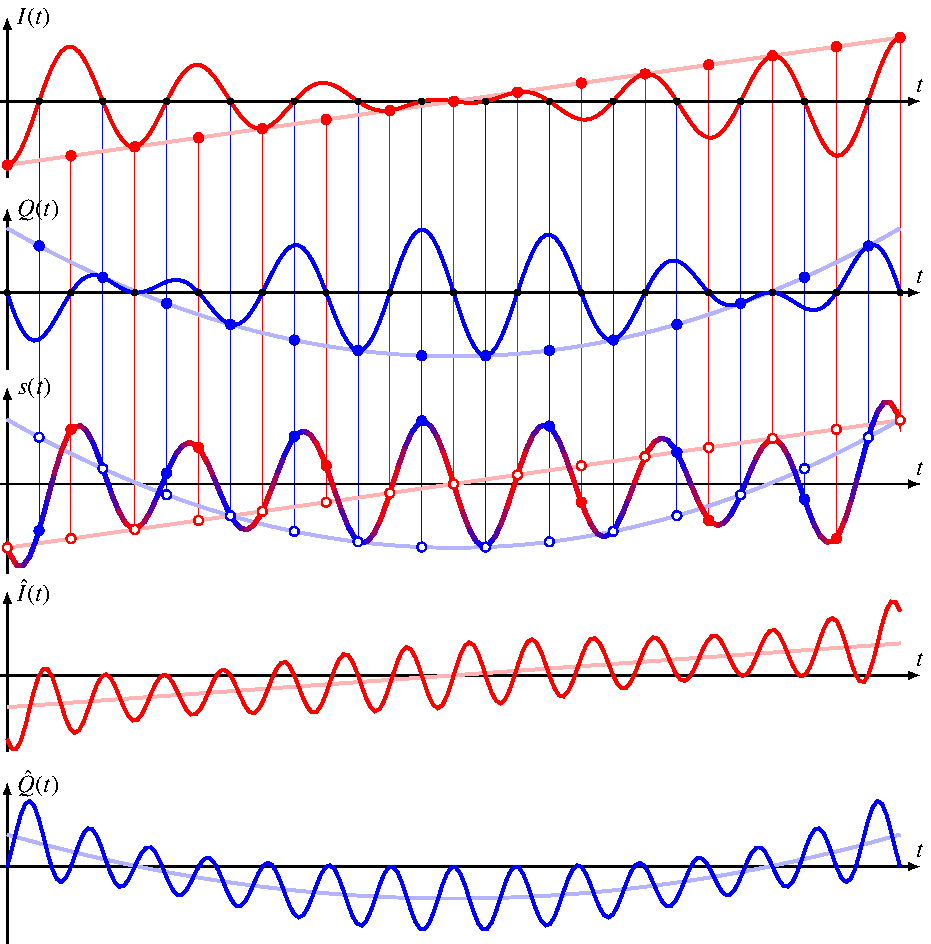
\includegraphics{applications/qam/images/sep.pdf}
\caption{Rekonstruktion der Signale $I(t)$ und $Q(t)$ (oberste zwei Graphen)
aus der Summe $s(t) = I(t)\cos\omega t - Q(t)\sin\omega t$ (Mitte).
Die Nullstellen von $\cos\omega t$ sind durch feine blaue Linien 
dargestellt, die Nullstellen von $\sin\omega t$ durch feine rote Linien.
Der Graph von $s(t)$ ist jeweils mit der Farbe eingefärbt, die den
dominanten Beitrag repräsentiert.
Blaue Segmente im Graphen von $s(t)$ bedeuten, dass vor allem der Wert
von $Q(t)$ zum Wert beiträgt, dies geschieht in der Umgebung von
Nullstellen von $\cos\omega t$, in den roten Segmenten ist es der Wert von
$I(t)$, welcher dominiert während $\sin\omega t$ eine Nullstelle durchläuft.
Fette Punkte auf dem Graphen von $s(t)$ markieren Punkte bei den
genannten Nullstellen.
Die leeren Punkte sind Werte von $s(t)$, die um das Vorzeichen des
Trägeres korrigiert wurden, sie liegen genau auf dem Graphen der
ursprünglichen Signale $I(t)$ und $Q(t)$.
Die untersten zwei Graphen zeigen die rekonstruierten Signale
$\hat{I}(t)=s(t) \cos\omega t$ und $\hat{Q}(t) = -s(t) \sin\omega t$, 
welche in Abschnitt~\ref{subsection:demodulation} erklärt werden.
\label{figure:qam:sep}}
\end{figure}

Einzelne Werte der Funktionen $I(t)$ und $Q(t)$ können aber aus der Summe
\[
s(t)
=
I(t)\cos\omega t - Q(t)\sin\omega t
\]
rekonstruiert werden.
An den Stellen $t = k\pi/\omega$ für $k\in\mathbb Z$ verschwindet
der Faktor $\sin\omega t$,
so dass an diesen Stellen der zweite Summand in $s(t)$ wegfällt.
Ebenso wird der erste Summand an den Stellen
$t = (k+\frac12)\pi/\omega$ verschwinden.
Dieser Sachverhalt ist in Abbildung~\ref{figure:qam:sep} dargestellt.
Es ist also
\[
s\biggl(k\cdot \frac{\pi}{2\omega}\biggr)
=
\begin{cases}
I(k\cdot \frac{\pi}{2\omega})\cdot(-1)^{\frac{k}2}
&\qquad \text{$k$ gerade,}\\[5pt]
Q(k\cdot \frac{\pi}{2\omega})\cdot(-1)^{\frac{k-1}2}
&\qquad \text{$k$ ungerade.}
\end{cases}
\]
Zu Zeitpunkten, die Vielfache von $\pi/2\omega$ sind, kann man also aus
$s(t)$ die Werte von $I(t)$ und $Q(t)$ ablesen.
Tatsächlich lernt man im Fach {\em Signale und Systeme}, dass man daraus
die Funktionen $I(t)$ und $Q(t)$ rekonstruieren kann, wenn sie keine
Frequenzkomponenten grösser als die Trägerfrequenz haben.
Die Summe $s(t)$ ist also etwas, was man potentiell drahtlos übermitteln
kann, und woraus man die Komponenten $I(t)$ und $Q(t)$ zurückgewinnen kann.
Man nennt dieses Modulationsverfahren {\em Quadratur-Amplituden-Modulation}.

Da wir über das nötige signaltheoretische Wissen noch nicht verfügen,
müssen wir eine alternative, geometrische Methode suchen, wie wir
aus $s(t)$ die Komponenten $I(t)$ und $Q(t)$ wiedergewinnen können.
Das modulierte Signal $s(t)$ ist also nichts anderes als eine
Komponente eines Vektors, der entsteht indem $\vec{v}(t)$ mit sehr grosser
Winkelgeschwindigkeit $\omega$ um den Ursprung gedreht wird.
Wir sind aber insofern nicht weiter, dass wir $I(t)$ und $Q(t)$ noch nicht
rekonstruieren können.




%
% demodulation.tex -- Demodulation von QAM
%
% (c) 2020 Prof Dr Andreas Müller, Hochschule Rapperswil
%
\subsection{Demodulation
\label{subsection:demodulation}}
Die modulierten Komponenten $s(t)$ und $c(t)$ entstehen gemäss
\eqref{eqn:qam:modulation}
durch eine sehr rasche Drehung $D_{\omega t}\vec{v}(t)$
des Vektor $\vec{v}(t)$.
Da die Drehung durch eine Matrix beschrieben wird, können wir
sie auch wieder rückgängig machen, indem wir mit der inversen
Matrix
\[
D^{-1}_{\omega t} = D_{-\omega t}
=
\begin{pmatrix}
\phantom{-}\cos\omega t & \sin\omega t \\
         - \sin\omega t & \cos\omega t
\end{pmatrix}
\]
multiplizieren.
So finden wir
\[
D_{\omega t}^{-1}
\begin{pmatrix}s(t)\\c(t)\end{pmatrix}
=
D_{\omega t}^{-1}
D_{\omega t}^{\mathstrut}
\begin{pmatrix} I(t)\\Q(t)\end{pmatrix}
=
\begin{pmatrix}
I(t)\\
Q(t)
\end{pmatrix}.
\]
Es ist also klar, dass man aus $s(t)$ und $c(t)$ die ursprünglichen Signale
$I(t)$ und $Q(t)$ rekonstruieren kann.
Allerdings ist auch dies nicht wirklich eine Lösung des Problems.
Es ist immer noch notwendig, die beiden Funktionen $s(t)$ und $c(t)$
getrennt zu übertragen, um $I(t)$ und $Q(t)$ wiederzugewinnen.

\subsubsection{Demodulation mit Trigonometrie}
Wir suchen ein Verfahren, mit dem wir $I(t)$ und $Q(t)$ allein aus
$s(t)$ zurückgewinnen können.
Auch für dieses Problem suchen wir eine geometrische Lösung.
Wir gehen dazu von der Gleichung
\[
\vec{v}(t)
=
D_{-\omega t}\underbrace{D_{\omega t}
\vec{v}(t)}_{=\begin{pmatrix}s(t)\\c(t)\end{pmatrix}}
\]
aus.
Die Tatsache, dass wir $c(t)$ nicht übertragen wollen, können wir dadurch
abbilden, dass wir in der Gleichung eine Projektionsmatrix $P$
verwenden, um die Komponeten $c(t)$ zu unterdrücken:
\[
P=\begin{pmatrix}1&0\\0&0\end{pmatrix}
\qquad\Rightarrow\qquad
P\begin{pmatrix}s(t)\\c(t)\end{pmatrix}
=
\begin{pmatrix}s(t)\\0\end{pmatrix}.
\]
Durch diese Änderung wird man natürlich nicht mehr $I(t)$ und $Q(t)$ 
zurückgewinnen können, stattdessen wird man modifizierte Funktionen
$\hat{I}(t)$ und $\hat{Q}(t)$ erhalten.
Das ganze Übertragung\-system könnte daher mit dem Matrizenprodukt
\[
\begin{pmatrix}
\hat{I}(t)\\
\hat{Q}(t)
\end{pmatrix}
=
D_{-\omega t} \begin{pmatrix}s(t)\\0\end{pmatrix}
=
D_{-\omega t} P D_{\omega t}\vec{v}(t)
\]
beschrieben werden.
Wegen
\[
D_{-\omega t}P
=
\begin{pmatrix}
\phantom{-}\cos\omega t & 0 \\
         - \sin\omega t & 0
\end{pmatrix}
\]
bedeutet dies
\begin{align*}
\hat{I}(t) &= \phantom{-}\cos\omega t s(t),\\
\hat{Q}(t) &= -\sin\omega t s(t).
\end{align*}
Wir bezeichnen den Vektor mit diesen Komponenten als
\[
\hat{v}(t) = \begin{pmatrix}\hat{I}(t)\\\hat{Q}(t)\end{pmatrix}.
\]
Der Vektor ist also das, was von der Rekonstruktion nach dem Wegfallen
der Komponente $c(t)$ noch übrig bleibt.

Wie unterscheiden sich $\hat{I}(t)$ und $\hat{Q}(t)$ von $I(t)$ und $Q(t)$?
Dazu berechnen wir
\begin{align*}
D_{-\omega t}PD_{\omega t}
&=
\begin{pmatrix}
\phantom{-}\cos\omega t & \sin\omega t \\
         - \sin\omega t & \cos\omega t
\end{pmatrix}
\begin{pmatrix} 1 & 0 \\ 0 & 0 \end{pmatrix}
\begin{pmatrix}
\cos\omega t &          - \sin\omega t \\
\sin\omega t & \phantom{-}\cos\omega t
\end{pmatrix}
\\
&=
\begin{pmatrix}
 \cos^2\omega t           & -\cos\omega t \sin\omega t \\
-\cos\omega t \sin\omega t&\sin^2\omega t
\end{pmatrix}
=
\frac12
\begin{pmatrix}
1+\cos 2\omega t &  -\sin 2\omega t \\
 -\sin 2\omega t & 1-\cos 2\omega t
\end{pmatrix}
\\
&=
\frac12 E + \frac12
\begin{pmatrix}
 \cos 2\omega t & -\sin 2\omega t \\
-\sin 2\omega t & -\cos 2\omega t
\end{pmatrix}.
\end{align*}
Im zweitletzten Schritt haben wir die Doppelwinkelformeln für
die trigonometrischen Funktionen verwendet.
Nach der Rekonstruktion bleiben also zwei Terme
\[
\hat{v}(t)
=
\frac12\vec{v}(t)
+
\frac12
\begin{pmatrix}
\phantom{-}\cos 2\omega t & -\sin 2\omega t \\
         - \sin 2\omega t & -\cos 2\omega t
\end{pmatrix}\vec{v}(t).
\]
Der erste Term ist bis auf den Faktor $\frac12$ der gesuchte
Vektor $\vec{v}(t)$.
Doch was ist der zweite Term?
Die Matrix kann man auch schreiben als
\begin{align*}
\begin{pmatrix}
\phantom{-}\cos2\omega t&-\sin2\omega t\\
         - \sin2\omega t&-\cos2\omega t
\end{pmatrix}
&=
\underbrace{
\begin{pmatrix}
1& 0\\
0&-1
\end{pmatrix}}_{\displaystyle = S}
\begin{pmatrix}
\cos2\omega t &          - \sin2\omega t \\
\sin2\omega t & \phantom{-}\cos2\omega t
\end{pmatrix}
=
\begin{pmatrix}
1& 0\\
0&-1
\end{pmatrix}
D_{2\omega t},
\end{align*}
bis auf die Spiegelungsmatrix $S$ handelt es sich also wieder um eine
Drehung, allerdings mit der doppelten Frequenz.
Beides zusammen kann kurz als
\begin{equation}
\hat{v}(t)
=
\frac12 \vec{v}(t)
+
\frac12 SD_{2\omega t}\vec{v}(t)
\label{eqn:qam:filter}
\end{equation}
geschrieben werden.

Die untersten zwei Graphen in Abbildung~\ref{figure:qam:sep} zeigen
die Komponenten $\hat{I}(t)$ und $\hat{Q}(t)$.
Es ist gut erkennbar, wie sie sich zusammensetzen aus $\frac12I(t)$ 
bzw.~$\frac12Q(t)$ überlagert mit einer Schwingung mit der doppelten
Frequenz des Trägers.

\subsubsection{Demodulation mit Matrixalgebra}
In der vorangegangenen Herleitung der Formel~\eqref{eqn:qam:filter}
haben wir ausgiebig von trigonometrischen Formeln Gebrauch gemacht.
Wir können die Formel aber auch auf eine viel geometrischere Art verstehen.
Dazu schreiben wir die Projektionsmatrix $P$ als eine Summe
\[
P
=
\begin{pmatrix}1&0\\0&0\end{pmatrix}
=
\begin{pmatrix}\frac12+\frac12&0\\0&\frac12-\frac12\end{pmatrix}
=
\frac12\begin{pmatrix}1&0\\0&1\end{pmatrix}
+
\frac12\begin{pmatrix}1&0\\0&-1\end{pmatrix}
=
\frac12E+\frac12S.
\]
Damit wird
\[
D_{-\omega t}PD_{\omega t}
=
\frac12D_{-\omega t}ED_{\omega t}
+
\frac12D_{-\omega t}SD_{\omega t}
=
\frac12E
+
\frac12D_{-\omega t}SD_{\omega t}.
\]
Wir wollen das Produkt $D_{-\omega t}S$ geometrisch verstehen und
modifizieren.
Die Matrix $S$ spiegelt Vektoren an der $I$-Achse, die Matrix $D_{-\omega t}$
dreht Vektoren um den Winkel $-\omega t$
(Abbildung~\ref{figure:qam:spiegelung}).
\begin{figure}
\centering
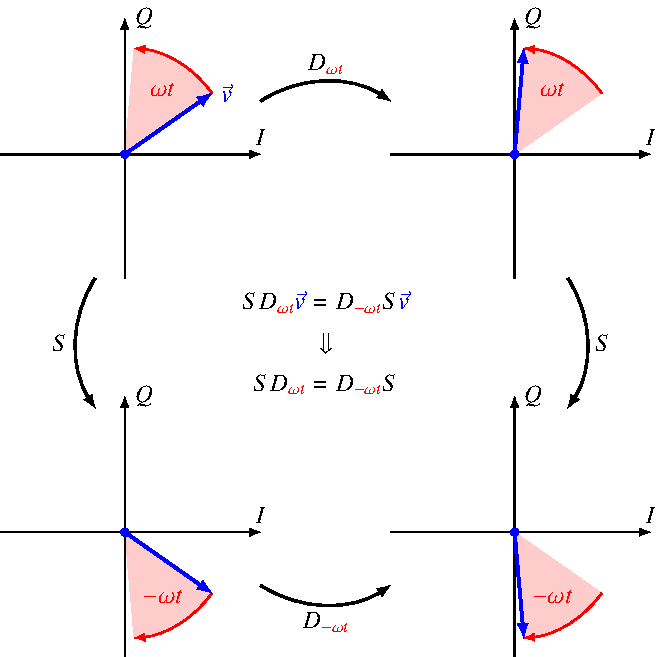
\includegraphics{applications/qam/images/spiegelung.pdf}
\caption{Vertauschungsregel für die Drehmatrizen $D_{\pm\omega t}$ und
die Matrix $S$ der Spiegelung an der $I$-Achse.
\label{figure:qam:spiegelung}}
\end{figure}
Zusammen bewirken sie dasselbe wie eine Drehung um $\omega t$ gefolgt
von einer Spiegelung an der $I$-Achse, also
\[
D_{-\omega t}S=SD_{\omega t}.
\]
Damit erhalten wir
\[
D_{-\omega t}PD_{\omega t}
=
\frac12E + \frac12 SD_{2\omega t},
\]
woraus wieder die Formel~\eqref{eqn:qam:filter}
für $\hat{v}(t)$ folgt.

\subsubsection{Filterung des Trägers}
\begin{figure}
\centering
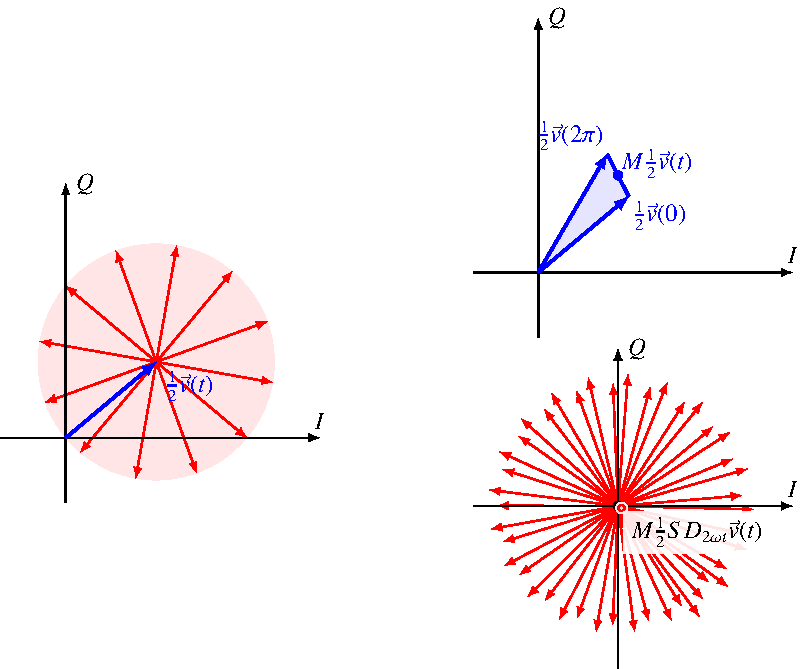
\includegraphics{applications/qam/images/filter.pdf}
\caption{Filterung des Trägers aus~\eqref{eqn:qam:filter}
links für ein konstantes Signal $\vec{v}(t)=\vec{v}(0)$, rechts
für ein langsam veränderliches Signal.
Zur besseren Lesbarkeit sind rechts die Terme
$\frac12\vec{v}(t)$ oben und $\frac12SD_{2\omega t}\vec{v}(t)$
unten getrennt.
Der Mittelwerte $\mathcal{M}\frac12SD_{2\omega t}$ ist der Beitrag des
zweiten Terms zum Mittelwert und sehr nahe beim Nullpunkt,
die Mittelung über ein Periodenintervall des Trägers bringt die
Trägerkomponente also fast vollständig zum Verschwinden.
\label{figure:qam:filter}}
\end{figure}
Gehen wir davon aus, dass die Bewegung des Vektors $\vec{v}(t)$ in
der $I$-$Q$-Ebene sehr viel langsamer ist als die Drehung mit der
Winkelgeschwindigkeit $2\omega$, dann können wir den zweiten Term
näherungsweise eliminieren.
Um dies zu verstehen, nehmen wir an, dass $\vec{v}(t)$ während eines
Zeitintervalls der Länge $L=\pi/\omega$ konstant ist ist.
Wir bezeichnen Mittelwerte über das Intervall mit dem Buchstaben $\mathcal{M}$.
Wir beachten dann, dass der zweite Term in \eqref{eqn:qam:filter}
für dieses Zeitintervall die gleichförmige, ganze Drehung des Vektors
um den Nullpunkt beschreibt.
Der Mittelwert des zweiten Terms über das Intervall verschwindet daher:
\[
\mathcal{M}\frac12SD_{2\omega t}\vec{v}(t)
=
0
\]
(siehe auch Abbildung~\ref{figure:qam:filter} links).
Der erste Term von \eqref{eqn:qam:filter} ist während des Intervalls
konstant, ihr Mittelwert ist daher
\[
\mathcal{M}\frac12\vec{v}(t)
=
\frac12\vec{v}(t).
\]
Wir finden daher den Mittelwert
\[
\mathcal{M}\hat{v}(t)
=
\frac12\vec{v}(t),
\]
bis auf den Faktor $\frac12$ wird also $\vec{v}(t)$ durch die Mittelwertbildung
rekonstruiert.
Verändert sich $\vec{v}(t)$ während des Intervalls um einen Betrag
kleiner als $\varepsilon$ (Abbildung~\ref{figure:qam:filter} rechts),
dann kommt ein Fehler hinzu, der ebenfalls
von der Grössenordnung $\varepsilon$ ist.

In praktischen Anwendungen ist die Frequenz des Trägers mehrere
Grössenordnungen grösser als die typischen Frequenzen in $I(t)$ 
und $Q(t)$, die Annahme, dass sich $\vec{v}(t)$ während einer halben
Trägerperiode nicht ändert, ist daher mit grosser Genauigkeit erfüllt.
Die Mittelwertbildung wird technisch mit Hilfe eines Tiefpassfilters
realisiert.

\subsubsection{Demodulationsfehler}
Bis jetzt sind wir davon ausgegangen, dass wir die Frequenz und die
Phase des Trägersignals genau kennen.
Doch dies ist nicht korrekt.
Die Demodulation erfolgt im Empfänger, wo die Matrix $D_{\omega t}$
neu erzeugt werden muss.
Dabei kann es zu Fehlern in der Frequenz kommen.
Die Demodulation erfolgt also mit einer Matrix $D_{\omega_rt}$
mit einer möglicherweise von der Sendefrequenz $\omega$
abweichenden Frequenz $\omega_r=\omega+\Delta\omega$.
Das decodierte Signal ist dann
\begin{equation}
\begin{aligned}
\hat{v}(t)
&=
D_{-\omega_rt}PD_{\omega t}\vec{v}(t)
=
D_{-(\omega+\Delta\omega)t} ({\textstyle\frac12}E+{\textstyle\frac12}S)
D_{\omega t}\vec{v}(t)
=
\frac12D_{-\Delta\omega t}\vec{v}(t)
+
\frac12D_{-(\omega+\Delta\omega)t}SD_{\omega t}\vec{v}(t)
\\
&=
\frac12 D_{-\Delta\omega t}\vec{v}(t)
+
\frac12 SD_{(\omega +\Delta\omega) t}D_{\omega t}\vec{v}(t)
=
\frac12 D_{-\Delta\omega t}\vec{v}(t)
+
\frac12 SD_{(2\omega +\Delta\omega) t}\vec{v}(t)
\end{aligned}
\label{eqn:qam:demoomegar}
\end{equation}
Bei der Filterung des Trägers verschwindet der zweite Term.
Die Demodulation liefert also nicht den Vektor $\vec{v}(t)$, vielmehr
rotiert der demodulierte Vektor mit der Winkelgeschwindigkeit $\Delta\omega$.

Korrekte Demodulation ist also nur möglich, wenn Sender und Empfänger exakt
die gleiche Frequenz verwenden.
Der Empfänger kann versuchen, die korrekte Frequenz aus dem empfangenen
Signal zu extrahieren, oder Sender und Empfänger können ein hochgenaues
Frequenznormal verwenden.
Ein Rubidium-Frequenznormal stellt eine Referenz-Frequenz mit einem
typischen relativen Fehler kleiner als $10^{-9}$ zur Verfügung.
Bei einem Trägersignal im typischen Bereich der Mobiltelefonie (Grössenordnung
$\sim 1\,\text{GHz}$) resultiert also weniger als eine Umdrehung von $\hat{v}(t)$
pro Sekunde.

Selbst wenn Sender und Empfänger hochgenaue Frequenzreferenzen verwenden,
wenn man also annehmen darf, dass $\omega_r=\omega$,
ist noch nicht sichergestellt, dass auch die Phase übereinstimmt.
Die Demodulation könnte mit einer um den Winkel $\delta$
phasenverschobenen Drehmatrix $D_{\omega t+\delta}$ erfolgen.
Die selbe Rechnung wie in \eqref{eqn:qam:demoomegar} liefert dann
\[
\hat{v}(t)
=
\frac12D_{-\delta}\vec{v}(t)
+
\frac12SD_{\delta+2\omega t}\vec{v}(t).
\]
Bei der Filterung fällt auch hier der zweite Term weg, der demodulierte
Vektor ist aber um den Winkel $-\delta$ verdreht.
Um dies zu vermeiden muss der Sender dem Empfänger die genaue Phase
irgendwie mitteilen.
Technische Möglichkeiten dazu werden in den nachstehenden Beispielen
kurz angesprochen.








%
% beispiele.tex
%
% (c) 2020 Prof Dr Andreas Müller, Hochschule Rapperswil
%
\subsection{Beispiele
\label{subsection:qam:beispiele}}
Die Quadratur-Amplituden-Modulation ermöglicht, im Vergleich zur
Trägerfrequenz langsam veränderliche zweidimensionale Signale zu
übertragen und wieder zu rekonstruieren.
Der besondere Nutzen dieser Technik ist jedoch, dass sie viele
ältere Modulationsverfahren als Spezialfälle enthält, wie in
diesem Abschnitt gezeigt werden soll.

\subsubsection{Amplitudenmodulation}
{\em Amplitudenmodulation} konnten wir verstehen, bevor wir $Q(t)$ kannten,
sie ist der Spezialfall $Q(t)=0$.
Für ein Audiosignal $A(t)$ mit $A(t)<1$ wird $I(t)=1+A(t)$ verwendet.
Das in Europa weitgehend bereits durch Digitalradio ersetzte 
Mittelwellenradio (AM) verwendet Amplitudenmodulation.
Bis 2025 werden in Europa alle Radiostationen digitalisiert, damit
wird AM für den Rundfunk aussterben.

\subsubsection{Phasenmodulation}
\begin{figure}
\centering
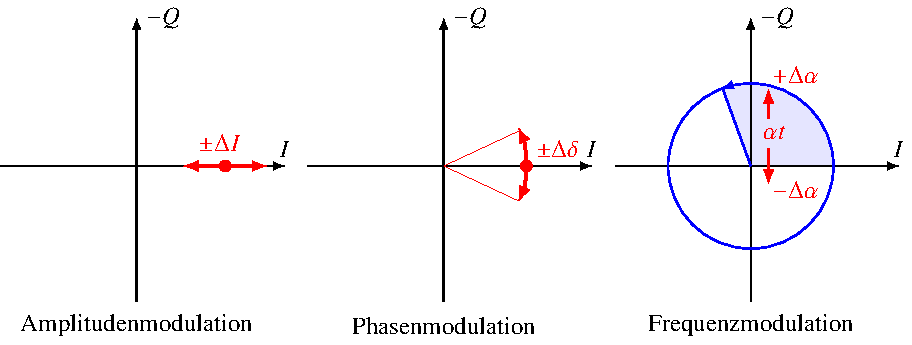
\includegraphics{applications/qam/images/amfmpm.pdf}
\caption{Amplitudenmodulation (links), Phasenmodulation (mitte) und
Frequenzmodulation in der $I$-$Q$-Ebene.
Frequenzmodulation ensteht durch eine Drehung in der $I$-$Q$-Ebene
mit der Kreisfrequenz der gewünschten Frequenzänderung.
\label{qam:figure:amfmpm}}
\end{figure}
Statt der Amplitude kann auch die Phase des Trägersignals moduliert werden.
Dazu muss $\omega t$ ersetzt werden durch $\omega t + \delta$.
Der konstante unmodulierte Vektor $\vec{v}_0$ in der $I$-$Q$-Ebene erzeugt
das modulierte Signal
\begin{align*}
D_{\omega t + \delta}
\vec{v}_0
&=
D_{\omega t}\underbrace{D_{\delta} \vec{v}_0}_{\displaystyle=\vec{v}(t)}.
\end{align*}
Eine Phasenänderung um den Winkel $\delta$ entsteht also dadurch, dass
man den Vektor $\vec{v}_0$ in der $I$-$Q$-Eben um $\delta$ dreht.
Dieses Modulationsverfahren heisst {\em Phasenmodulation}.
Abbildung~\ref{qam:figure:amfmpm} zeigt in der Mitte die Transformation
in der $I$-$Q$-Ebene, die Phasenmodulation bewirkt.

Mit reiner Amplitudenmodulation lässt sich kein Stereosignal übertragen.
Sind $L(t)$ und $R(t)$ die beiden Stereokanäle, dann erfolgt die
Amplitudenmodulation typischerweise mit $I(t)=1+L(t)+R(t)$,
wobei man wieder $L(t)+R(t)<1$ voraussetzen muss.
Ein reiner AM-Empfänger wird also nur das Audio-Signal $A(t)=L(t) + R(t)$
empfangen.

Um die Stereoinformation zu übermitteln, muss zusätzlich die Differenz
$L(t)-R(t)$ übermittelt werden.
Das C-QUAM Verfahren ({\bf C}ompatible {\bf Qu}adrature {\bf A}mplitude
{\bf M}odulation) verwendet dafür $Q(t)=L(t)-R(t)$.
Man darf annehmen, dass $L(t)-R(t)$ klein ist.
Dann befinden sich die Punkte $(I(t),Q(t))$ immer in der
Nähe der $I$-Achse, was sich in einer kleinen Verschiebung
\[
\delta = \arctan\frac{Q(t)}{I(t)} = \arctan\frac{L(t)-R(t)}{1+L(t)+R(t)}
\]
der Phase des übermittelten Signals äussert.
Der Betrag des Vektors $\vec{v}(t)$ ist dagegen
\begin{align*}
|\vec{v}(t)|
&=
\sqrt{
(1+L(t)+R(t))^2
+
(L(t)-R(t))^2
}
=
(1+L(t)+R(t))
\sqrt{
1+
\biggl(
\frac{L(t)-R(t)}{1+L(t)+R(t)}\biggr)^2
}
\\
&\simeq 1+L(t)+R(t),
\end{align*}
weil der zweite Summand unter der Wurzel klein ist.
Die $Q$-Komponente ändert also nicht wirklich etwas am Signal, welches
ein AM-Empfänger empfängt.

Um dem Emfpänger zu signalisieren, dass eine Stereoübertragung
vorliegt, wird $Q(t)$ zusätzlich ein Pilotton von 25\,Hz hinzugefügt.
Da nicht C-QUAM-taugliche Empfänger die Phasenschwankungen nicht erkennen
können, werden sie vom Pilotton auch nicht gestört.

\subsubsection{Frequenzmodulation}
Bei der {\em Frequenzmodulation} des UKW-Radios wird die Trägerfrequenz
im Takt des zu übertragenden Tonsignals verändert.
Lässt sich dies auch mit Hilfe der Signale $I(t)$ und $Q(t)$
beschreiben?
Welche Funktionen $I(t)$ und $Q(t)$ muss man wählen?

Ist das zu übertragende Audiosignal $0$, dann wird nur der unveränderte
Träger ausgestrahlt.
Dies lässt sich dadurch erreichen, dass man für $\vec{v}(t)$ den
konstanten Vektor $\vec{v}(t)=\vec{v}_0=(1,0)^t$ wählt.

Das ausgestrahlte Signal $s(t)$ entsteht als erste Komponente
des Vektors $D_{\omega t}\vec{v}(t)$.
Für konstantes $\vec{v}(t)=\vec{v}_0$ oszilliert es mit der Kreisfrequenz
$\omega$.
Will man, dass es schneller oszilliert, dann muss die Frequenz $\omega$
erhöht werden.
Möchte man die Frequenz um $\alpha$ steigern, dann muss man $\omega$
durch $\omega+\alpha$ ersetzen.
Das modulierte Signal ist dann
\[
\begin{pmatrix}
s(t)\\c(t)
\end{pmatrix}
=
D_{(\omega+\alpha)t} \vec{v}_0
=
D_{\omega t} \underbrace{D_{\alpha t} \vec{v}_0}_{\displaystyle=\vec{v}(t)}.
\]
Dies ist gleichbedeutend damit, dass man den Vektor $\vec{v}_0$ in der
$I$-$Q$-Ebene mit der Winkelgeschwindigkeit $\alpha$ dreht und so
$\vec{v}(t)$ erhält.
Daraus liest man ab, dass für die Signale $I(t)$ und $Q(t)$
\begin{equation}
\begin{pmatrix}I(t)\\Q(t)\end{pmatrix}
=
D_{\alpha t}\vec{v}_0
\qquad\Rightarrow\qquad
\left\{
\quad
\begin{aligned}
I(t)&=\cos\alpha t\\
Q(t)&=\sin\alpha t
\end{aligned}
\right.
\end{equation}
gilt.
Insbesondere kann man auch die Frequenzmodulation mit der
Quadratur-Amplituden-Modulation realisieren.
Abbildung~\ref{qam:figure:amfmpm} zeigt rechts symbolisch die
Kreisbewegung in der $I$-$Q$-Ebene, die Frequenzmodulation bewirkt.

\subsubsection{Analoges Farbfernsehen}
Die Entwicklung des analogen Farbfernsehens sah sich vor die Aufgabe 
gestellt, zusätzlich zur bereits im Schwarz-Weiss-Fernsehen übertragenen
Helligkeit (Luminanz, Y) die Farbinformation zu übermitteln.
Üblich ist dabei die Verwendung des YUV-Farbraumes, für den die zusätzlichen
Signale $U=R-Y$ und $V=B-Y$ benötigt werden, welche die Farbinformation
codieren.
Für ein farbloses Bild sind $U=0$ und $V=0$.

Das Problem ist also, zusätzlich zum Luminanzbild, welches bereits
amplitudenmoduliert übertragen wird, den Farbvektor $(U,V)^t$ zu
übertragen.
Es liegt daher nahe, dafür die Quadratur-Amplituden-Modulation zu
verwenden.
Im in Europa üblichen PAL-System wurde für den Träger für das Farbsignal
die Frequenz 4.43361875\,MHz verwendet.
Da ein Phasenfehler im Empfänger zu einer Drehung des Farbvektors
und damit zu einer auffälligen Verschiebung der Farben auf dem Farbkreis
führen würde, muss der Sender dem Empfänger die genaue Phase mitteilen.
Am Anfang jeder Zeile wird daher eine etwa zehn Perioden langer ``PAL-Burst''
übermittelt, den der Empfänger dazu verwenden kann, die Phase des
Farbträgers zu bestimmen.

Zusätzlich invertiert das PAL-System die Phase des Farbträgers
aufeinanderfolgender Zeilen, so dass sich Farbfehler durch Phasenfehler
auf aufeinanderfolgenden Zeilen wegmitteln.
Im PAL-System steht also Farbinformation jeweils nur für Paare von Zeilen
zur Verfügung und nur mit einer Dichte, die durch die Frequenz des Farbträgers
begrenzt ist.
Die effektive Farbauflösung eines PAL-Farbfernsehbildes ist daher halb so
gross wie die Helligkeitsauflösung.
Da auch die Farbauflösung des menschlichen Auges kleiner ist als die
Helligkeitsauflösung, ist diese Einschränkung des Systems von Auge nicht 
erkennbar.

\subsubsection{FSK und PSK}
Für die digitale Signalübertragung braucht man minimal die Fähigkeit,
zwei Zustände zu übermitteln, die man aber exakt wiedererkennnen können muss.
Frequency-Shift-Keying (FSK) ist ein Verfahren, welches zwei digitale Zustände
durch verschiedene Frequenzen codiert, es ist also ein
Frequenzmodulationsverfahren, von dem im vorangegangenen Abschnitt
bereits gezeigt wurde, wie es mit der Quadratur-Amplituden-Modulation
realisierbar ist.

Phase-Shift-Keying (PSK) verwendet stattdessen eine Phasenverschiebung
des Tragersignals.
Eine Phasenverschiebung um den Winkel $\varphi$ kann realisiert werden,
indem man eine Drehung um den Winkel $\varphi$ vorschaltet, also die
Drehmatrix $D_{\varphi}$ einfügt.
Besonders einfach ist eine Phasenverschiebung um den Winkel
$\varphi=180^\circ$, 
\[
D_{\varphi}
=
\begin{pmatrix}
\cos180^\circ&          - \sin180^\circ \\
\sin180^\circ& \phantom{-}\cos180^\circ
\end{pmatrix}
=
-E.
\]
Diese Phasenverschiebung wird also dadurch realisiert, dass man das
Vorzeichen von $I$ und $Q$ ändert.
Verwendet man den Vektor $(1,0)^t$ zur Codierung einer logischen
$\texttt{0}$, dann codiert der Vektor $(-1,0)^t$ eine logische $\texttt{1}$.
Auch PSK ist also mit Quadratur-Amplituden-Modulation realisierbar.

\subsubsection{Quantisierte QAM}
Mit Quadratur-Amplituden-Modulation lässt sich ein beliebiger Vektor
in der $I$-$Q$-Ebene übertragen.
Bei PSK wurden nur die Punkte $(1,0)$  und $(-1,0)$ in der $I$-$Q$-Ebene
verwendet.
Nach der Demodulation erhält man Vektoren, die wegen Fehlern nicht
exakt mit den ursprünglichen Vektoren übereinstimmen.
Da man aber nur die beiden logischen Zustände unterscheiden können muss,
kann man alle Vektoren mit $I>0$ als logische \texttt{0} decodieren
und Vektoren mit $I<0$ als logische \texttt{1}.

Statt nur zwei Zustände \texttt{0} und \texttt{1} zu codieren, könnte man
ein grössere Zahl von Punkten in der $I$-$Q$-Ebene verwenden, wie in
Abbildung~\ref{figure:qam:konstellation} dargestellt.
Die Punkte werden auch {\em Symbole} genannt.
Ein empfangener Vektor wird wegen Übertragungsfehlern nicht exakt mit
dem ursprünglichen Vektor übereinstimmen.
Zur Decodierung suchen wir dasjenige Symbol, welches dem Vektor am
nächsten liegt.
Man teilt also die Ebene in Teilgebiete $T_{\vec{v}_k}\subset \mathbb R^2$
zu jedem Symbol $\vec{v}_k$ auf.
Fällt der empfangene Vektor $\hat{v}$ in das Teilgebiet des Symbols
$\vec{v}_k$, also $\hat{v}\in T_{\vec{v}_k}$, dann decodieren wir ihn
als das Symbol $\vec{v}_k$.

\begin{figure}
\centering
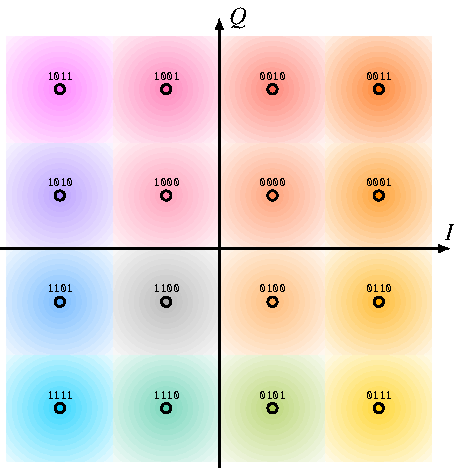
\includegraphics{applications/qam/images/konstellation.pdf}
\caption{Konstellationsdiagramm für quantisierte QAM mit 16 verschiedenen
Symbolen.
Mit jedem Symbol werden vier Bit codiert.
Zu jedem Symbol gehört ein quadratisches Gebiet gleicher Farbe.
Fällt der empfangene Vektor in eines dieser Gebiete, wird er als
das zugehörige Symbol decodiert.
\label{figure:qam:konstellation}}
\end{figure}

Im Beispiel der Abbildung~\ref{figure:qam:konstellation} können 16 
verschiedene Vektoren unterschieden werden, die man mit vierstelligen
Binärzahlen identifizieren kann.
Mit jedem Symbol werden also vier Bit übertragen.
Dieses Verfahren heisst auch 16-QAM und wird bei DVB-T verwendet.

Die Punkte-Menge $\vec{v}_k$ heisst auch die {\em Konstellation}
des Verfahrens.
Durch feinere Aufteilung können mehr Bits pro Symbol übertragen werden,
wie in Tabelle~\ref{table:qam:xqam} zusammengstellt.
Abbildung~\ref{figure:qam:analyzer} zeigt, wie sich die Messung eines 256-QAM 
Signals auf einem Vector Signal Analyzer darstellt.

Für ungerade Potenzen von $2$ kann das Konstellationsdiagramm kein
Quadrat sein.
Für $k$ ungerade kann man aber $2^k$ Punkte erhalten, indem man
dem Quadrat der $2^{k-1}$ Punkte der Konstellation von $2^{k-1}$-QAM
vier Rechtecke mit jeweils $2^{k-1}/4=2^{k-3}$ Punkten hinzugefügt, daraus
ergibt sich eine Konstellation mit
$2^{k-1}+4\cdot 2^{k-3}=2^{k-1}+2^{k-1}=2^k$
Punkten (Abbildung~\ref{qam:figure:qam-konstellation} Mitte).
In diesem hat das Konstellationsdiagramm also die Form
eines Kreuzes mit breite $2^{(k-1)/2}$ und Armlänge
$\frac32\cdot 2^{(k-1)/2}$.
Diese Konstellation wird manchmal auch Cross-QAM genannt.

\begin{table}
\centering
\begin{tabular}{rrcrl}
\hline
Bits&Symbole&Konstellation&Name&Anwendung\\
\hline
   2&      4&$  2\times   2$      &    4-QAM&DVB-S       \\
   4&     16&$  4\times   4$      &   16-QAM&V.29, DVB-T \\
   6&     64&$  8\times   8$      &   64-QAM&DVB-C, DVB-T\\
   8&    256&$ 16\times  16$      &  256-QAM&DVB-C       \\
  10&   1024&$ 32\times  32$      & 1024-QAM&            \\
  12&   4096&$ 64\times  64$      & 4096-QAM&DVB-C2, G.hn\\
  15&  32768&$128\times 256$ Kreuz&32767-QAM&ADSL        \\
\hline
\end{tabular}
\caption{Verschiedene Konstellationen für quantisierte QAM mit Anwendungen.
\label{table:qam:xqam}}
\end{table}

\begin{figure}
\centering
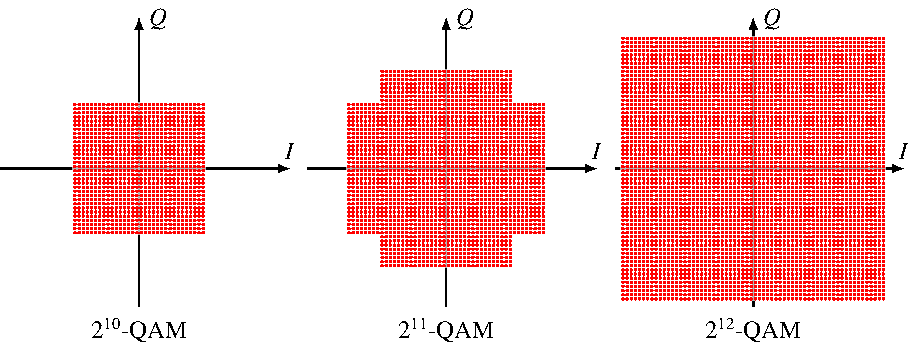
\includegraphics{applications/qam/images/qam.pdf}
\caption{Konstellationsdiagramme für $2^k$-QAM für verschiedene Werte von $k$.
\label{qam:figure:qam-konstellation}}
\end{figure}

\begin{figure}
\centering
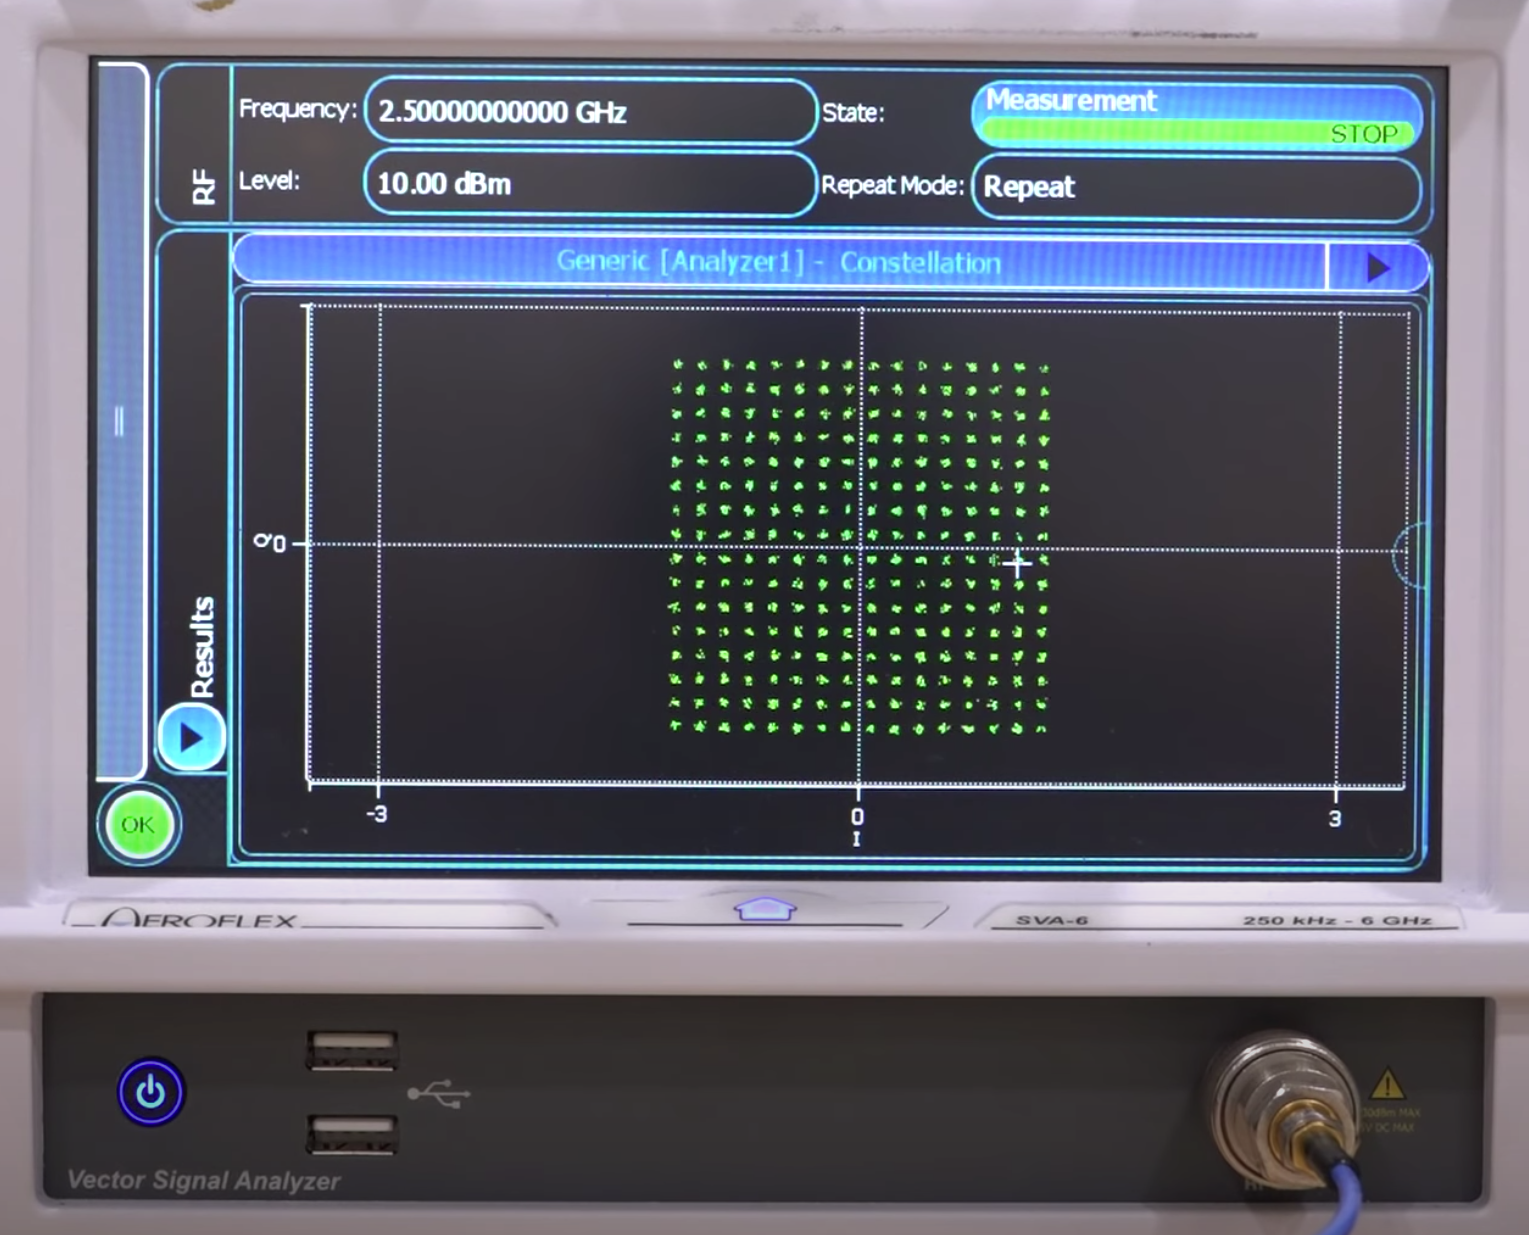
\includegraphics[width=1.0\hsize]{applications/qam/images/analyzer.png}
\caption{Messung des Konstellationsdiagramms eines 256-QAM Signals
mit einem Vector Signal Analyzer.
Man beachte die Beschriftung der Achsen mit \texttt{I} und \texttt{Q}.
(Ausschnitt aus dem Video \url{https://www.youtube.com/watch?v=uV3O3tpjmS8}
bei 26:36).
\label{figure:qam:analyzer}}
\end{figure}

\subsubsection{$n$-PSK}
Analog zum Vorgehen bei der quantisierten QAM kann auch PSK diskretisiert
werden.
Als Konstellationsdiagramm für $n$-PSK dienen $n$ Punkte auf einem Kreis,
die durch einen Winkel $2\pi/n$ getrennt sind.
In Abbildung~\ref{figure:qam:psk} ist das Konstellationsdiagramm für
$8$-PSK dargestellt.
\begin{figure}
\centering
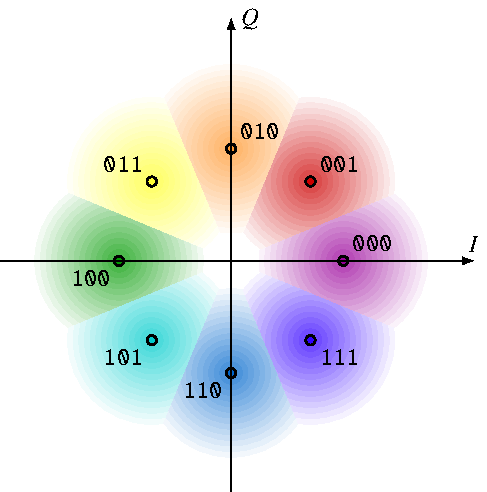
\includegraphics{applications/qam/images/psk.pdf}
\caption{Konstellationsdiagramm für 8-PSK 
\label{figure:qam:psk}}
\end{figure}

\subsubsection{Software Defined Radio}
Die vorangegangenen Beispiele haben illustriert, dass die
Quadratur-Amplituden-Modulation jedes besprochene Modulationsverfahren
realisieren kann.
Es ist nur nötig, einen Sender zu bauen, der Inputs $I(t)$ und $Q(t)$
entgegennimmt, die Modulation mit der Matrix $D_{\omega t}$ vornimmt
und das resultierende Signal $s(t)$ aussendet.
Auf der Empfängerseite braucht man eine physikalische Realisierung
der Matrix $D_{\omega_r t}$ und des Tiefpasses, der die demodulierten
Signal $\hat{I}(t)$ und $\hat{Q}(t)$ ausgibt.
Die Decodierung zum Beispiel als amplitudenmoduliertes Sprachsignal,
als frequenzmoduliertes Musiksignal oder als digitales 16-QAM-Signal
kann danach ausschliesslich in Software erfolgen.
Die Modulationsart eines solchen sogenannten {\em Software Defined Radio (SDR)}
wird also durch die Software definiert, welche die Signale $I(t)$ und $Q(t)$
erzeugt bzw.~die Signale $\hat{I}(t)$ und $\hat{Q}(t)$ analysiert.
SDR ermöglicht dem interessierten Hacker auch exotische Experimente,
wie das in Abbildung~\ref{qam:figure:digital} dargestellte fiktive
digitale Modulationsverfahren.

\begin{figure}
\centering
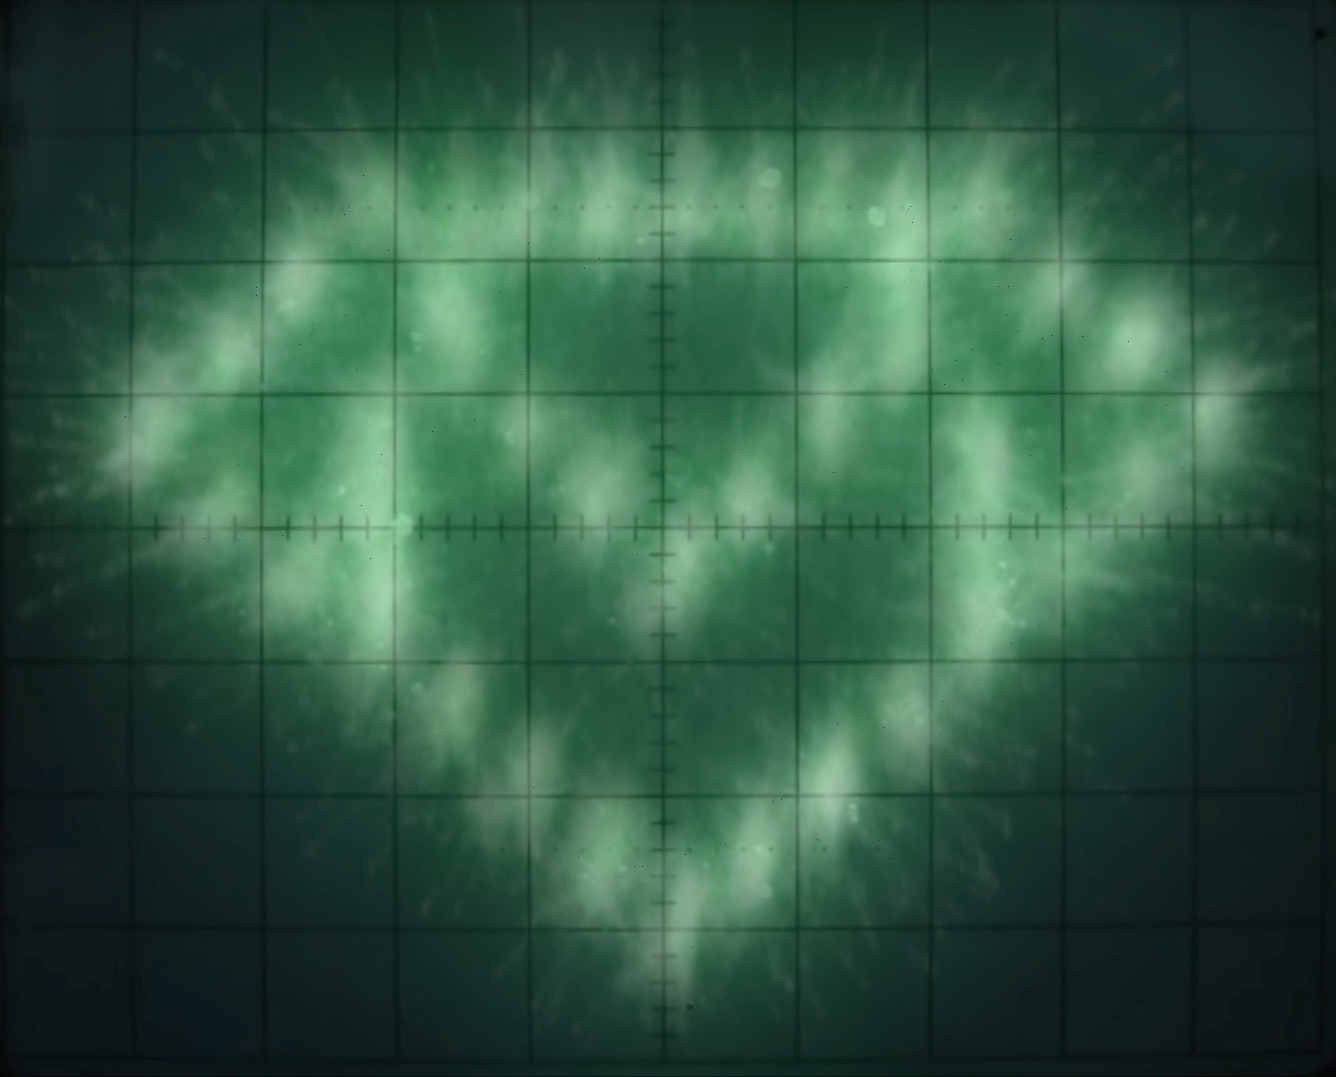
\includegraphics[width=0.7\hsize]{applications/qam/images/digital.jpg}
\caption{Konstellationsdiagramm für ein fiktives digitales
Modulationsverfahren, welches nur Punkte eines MathMan-Logos als
Symbole verwendet.
\label{qam:figure:digital}}
\end{figure}








